\documentclass[12pt]{article}

%%%%%%%%%%%%%%%%%%%%%%%%%%%%%%%%%%%%%%%%%
% Lachaise Assignment
% Structure Specification File
% Version 1.0 (26/6/2018)
%
% This template originates from:
% http://www.LaTeXTemplates.com
%
% Authors:
% Marion Lachaise & François Févotte
% Vel (vel@LaTeXTemplates.com)
%
% License:
% CC BY-NC-SA 3.0 (http://creativecommons.org/licenses/by-nc-sa/3.0/)
% 
%%%%%%%%%%%%%%%%%%%%%%%%%%%%%%%%%%%%%%%%%

%----------------------------------------------------------------------------------------
%	PACKAGES AND OTHER DOCUMENT CONFIGURATIONS
%----------------------------------------------------------------------------------------

\usepackage{amsmath,amsfonts,stmaryrd,amssymb} % Math packages

\usepackage{enumerate} % Custom item numbers for enumerations

\usepackage[ruled]{algorithm2e} % Algorithms

\usepackage[framemethod=tikz]{mdframed} % Allows defining custom boxed/framed environments

\usepackage{listings} % File listings, with syntax highlighting
\lstset{
	basicstyle=\ttfamily, % Typeset listings in monospace font
}

%----------------------------------------------------------------------------------------
%	DOCUMENT MARGINS
%----------------------------------------------------------------------------------------

\usepackage{geometry} % Required for adjusting page dimensions and margins

\geometry{
	paper=a4paper, % Paper size, change to letterpaper for US letter size
	top=2.5cm, % Top margin
	bottom=3cm, % Bottom margin
	left=2.5cm, % Left margin
	right=2.5cm, % Right margin
	headheight=14pt, % Header height
	footskip=1.5cm, % Space from the bottom margin to the baseline of the footer
	headsep=1.2cm, % Space from the top margin to the baseline of the header
	%showframe, % Uncomment to show how the type block is set on the page
}

%----------------------------------------------------------------------------------------
%	FONTS
%----------------------------------------------------------------------------------------

\usepackage[utf8]{inputenc} % Required for inputting international characters
\usepackage[T1]{fontenc} % Output font encoding for international characters

\usepackage{XCharter} % Use the XCharter fonts

%----------------------------------------------------------------------------------------
%	COMMAND LINE ENVIRONMENT
%----------------------------------------------------------------------------------------

% Usage:
% \begin{commandline}
%	\begin{verbatim}
%		$ ls
%		
%		Applications	Desktop	...
%	\end{verbatim}
% \end{commandline}

\mdfdefinestyle{commandline}{
	leftmargin=10pt,
	rightmargin=10pt,
	innerleftmargin=15pt,
	middlelinecolor=black!50!white,
	middlelinewidth=2pt,
	frametitlerule=false,
	backgroundcolor=black!5!white,
	frametitle={Command Line},
	frametitlefont={\normalfont\sffamily\color{white}\hspace{-1em}},
	frametitlebackgroundcolor=black!50!white,
	nobreak,
}

% Define a custom environment for command-line snapshots
\newenvironment{commandline}{
	\medskip
	\begin{mdframed}[style=commandline]
}{
	\end{mdframed}
	\medskip
}

%----------------------------------------------------------------------------------------
%	FILE CONTENTS ENVIRONMENT
%----------------------------------------------------------------------------------------

% Usage:
% \begin{file}[optional filename, defaults to "File"]
%	File contents, for example, with a listings environment
% \end{file}

\mdfdefinestyle{file}{
	innertopmargin=1.6\baselineskip,
	innerbottommargin=0.8\baselineskip,
	topline=false, bottomline=false,
	leftline=false, rightline=false,
	leftmargin=2cm,
	rightmargin=2cm,
	singleextra={%
		\draw[fill=black!10!white](P)++(0,-1.2em)rectangle(P-|O);
		\node[anchor=north west]
		at(P-|O){\ttfamily\mdfilename};
		%
		\def\l{3em}
		\draw(O-|P)++(-\l,0)--++(\l,\l)--(P)--(P-|O)--(O)--cycle;
		\draw(O-|P)++(-\l,0)--++(0,\l)--++(\l,0);
	},
	nobreak,
}

% Define a custom environment for file contents
\newenvironment{file}[1][File]{ % Set the default filename to "File"
	\medskip
	\newcommand{\mdfilename}{#1}
	\begin{mdframed}[style=file]
}{
	\end{mdframed}
	\medskip
}

%----------------------------------------------------------------------------------------
%	NUMBERED QUESTIONS ENVIRONMENT
%----------------------------------------------------------------------------------------

% Usage:
% \begin{question}[optional title]
%	Question contents
% \end{question}

\mdfdefinestyle{question}{
	innertopmargin=1.2\baselineskip,
	innerbottommargin=0.8\baselineskip,
	roundcorner=5pt,
	nobreak,
	singleextra={%
		\draw(P-|O)node[xshift=1em,anchor=west,fill=white,draw,rounded corners=5pt]{%
		Question \theQuestion\questionTitle};
	},
}

\newcounter{Question} % Stores the current question number that gets iterated with each new question

% Define a custom environment for numbered questions
\newenvironment{question}[1][\unskip]{
	\bigskip
	\stepcounter{Question}
	\newcommand{\questionTitle}{~#1}
	\begin{mdframed}[style=question]
}{
	\end{mdframed}
	\medskip
}

%----------------------------------------------------------------------------------------
%	WARNING TEXT ENVIRONMENT
%----------------------------------------------------------------------------------------

% Usage:
% \begin{warn}[optional title, defaults to "Warning:"]
%	Contents
% \end{warn}

\mdfdefinestyle{warning}{
	topline=false, bottomline=false,
	leftline=false, rightline=false,
	nobreak,
	singleextra={%
		\draw(P-|O)++(-0.5em,0)node(tmp1){};
		\draw(P-|O)++(0.5em,0)node(tmp2){};
		\fill[black,rotate around={45:(P-|O)}](tmp1)rectangle(tmp2);
		\node at(P-|O){\color{white}\scriptsize\bf !};
		\draw[very thick](P-|O)++(0,-1em)--(O);%--(O-|P);
	}
}

% Define a custom environment for warning text
\newenvironment{warn}[1][Warning:]{ % Set the default warning to "Warning:"
	\medskip
	\begin{mdframed}[style=warning]
		\noindent{\textbf{#1}}
}{
	\end{mdframed}
}

%----------------------------------------------------------------------------------------
%	INFORMATION ENVIRONMENT
%----------------------------------------------------------------------------------------

% Usage:
% \begin{info}[optional title, defaults to "Info:"]
% 	contents
% 	\end{info}

\mdfdefinestyle{info}{%
	topline=false, bottomline=false,
	leftline=false, rightline=false,
	nobreak,
	singleextra={%
		\fill[black](P-|O)circle[radius=0.4em];
		\node at(P-|O){\color{white}\scriptsize\bf i};
		\draw[very thick](P-|O)++(0,-0.8em)--(O);%--(O-|P);
	}
}

% Define a custom environment for information
\newenvironment{info}[1][Info:]{ % Set the default title to "Info:"
	\medskip
	\begin{mdframed}[style=info]
		\noindent{\textbf{#1}}
}{
	\end{mdframed}
}

\title{VE527: Assignment \#6} % Title of the assignment
\author{Name: Chang Meng\\Student ID:\@\texttt{118370910019}}
\date{\today}

\begin{document}

\maketitle

\section{(6\%) Prime Cover}
Given the following SOP Boolean expressions:
\[wxy+yz+w\bar{y}\bar{z}+\bar{w}x\bar{y}z\]

Is it a prime cover,
i.e., are all the cubes in that expression prime implicants?
Why or why not?\\

Answer:
No,
because $\bar{w}x\bar{y}z$ can be covered by a ``larger'' implicant $\bar{w}xz$.

\section{(10\%) Expand Operation in Espresso}
Suppose that we are optimizing an SOP Boolean expression $F(a, b, c, d)$ using the reduce-expand-irredundant loop.
Assume that we have just done a REDUCE step and we have an intermediate, non-prime 4-cube cover of $F$ as
\[F = \bar{a}b\bar{c}\bar{d} + b\bar{c}d + cd + bc\bar{d}\]

We want to perform an EXPAND operation on the cube $\bar{a}b\bar{c}\bar{d}$.
As we learned in lecture,
ESPRESSO does this by building a cover of the OFF-set for this current cover,
then building a blocking matrix for the cube we seek to expand,
and then computing a cover of this matrix,
which tells us how to grow this cube.\\

Apply the recipe and show the result of EXPAND\@.
For simplicity,
assume that the OFF-set of $F$ is given to you,
which is the following 3-cube cover
\[\bar{F} = \bar{b}\bar{d} + \bar{b}\bar{c} + a\bar{c}\bar{d}\]

(Hint: you can draw Karnaugh map to verify if your answer is correct.)\\

Answer:

The blocking matrix is:

\begin{center}
    \tabcolsep=8pt
    \begin{tabular}{|c|c|c|c|}
        \hline
        \diagbox{var}{cube} & $\bar{b}\bar{d}$ & $\bar{b}\bar{c}$ & $a\bar{c}\bar{d}$ \\
        \hline
        $\bar{a}$ & 0 & 0 & 1 \\
        $b$       & 1 & 1 & 0 \\
        $\bar{c}$ & 0 & 0 & 0 \\
        $\bar{d}$ & 0 & 0 & 0 \\
        \hline
    \end{tabular}
\end{center}

We can only cover the matrix with $\bar{a}$ and $b$,
the corresponding legal cube expansion is $\bar{a}b$.
Thre result after EXPAND this cube $\bar{a}b\bar{c}\bar{d}$ is
\[F = \bar{a}b + b\bar{c}d + cd + bc\bar{d}\]

\section{(10\%) Algebraic Division}
Condider the following two functions of variables $p$, $q$, $r$, $s$, $t$, $u$, $v$, $w$, $x$, $y$, $z$:
\[F=pt+xz+qt+pyz+rst+qyz+puvw+px+quvw+rsuvw\]
\[D=p+q+rs\]

Use the algebric division algorithm from class to compute $Q=F/D$ and the remainder $R$.

(Hint: you want to build the table as in the lecture slides:
one row for each cube in F\@;
one column for each cube in D\@;
do the cube-wise walk though $D$ and build up the partial quotient solution for $Q$ one column of this table at a time.
When you are done,
you can obtain the remainder $R$ from the computed quotient.)\\

Answer:

\begin{center}
    \tabcolsep=8pt
    \begin{tabular}{|c|c|c|c|}
        \hline
        $F$ cube & $D$ cube $p$ & $D$ cube $q$ & $D$ cube $rs$ \\
        \hline
        $pt$    & $t$   & $-$   & $-$   \\
        $xz$    & $-$   & $-$   & $-$   \\
        $qt$    & $-$   & $t$   & $-$   \\
        $pyz$   & $yz$  & $-$   & $-$   \\
        $rst$   & $-$   & $-$   & $t$   \\
        $qyz$   & $-$   & $yz$  & $-$   \\
        $puvw$  & $uvw$ & $-$   & $-$   \\
        $px$    & $x$   & $-$   & $-$   \\
        $quvw$  & $-$   & $uvw$ & $-$   \\
        $rsuvw$ & $-$   & $-$   & $uvw$ \\
        \hline
    \end{tabular}
\end{center}

\[Q=(t+yz+uvw+x)\cap{(t+yz+uvw)}\cap{(t+uvw)}=t+uvw\]
\[R=F-QD=F-(pt+puvw+qt+quvw+rst+rsuvw)=xz+pyz+qyz+px\]

\section{(20\%) Kerneling}
Here is a function represented in algebraic form:
\[F=abe+ace+de+abfg+acfg+dfg+bh+ch\]

Assume that the variable order is $a$, $b$, $c$, $d$, $e$, $f$, $g$, $h$.
Use the recursive kerneling algorithm discussed in the lecture,
and run the algorithm by han =d to extract all the kernels and their associated co-kernels from $F$.
Show all the co-kernel --- kernel pairs.
Also, show the level number of each kernel
(i.e., some kernel is a level-0 kernel,
some level is a level-1 kernel, etc.)\\

Answer:

\begin{center}
    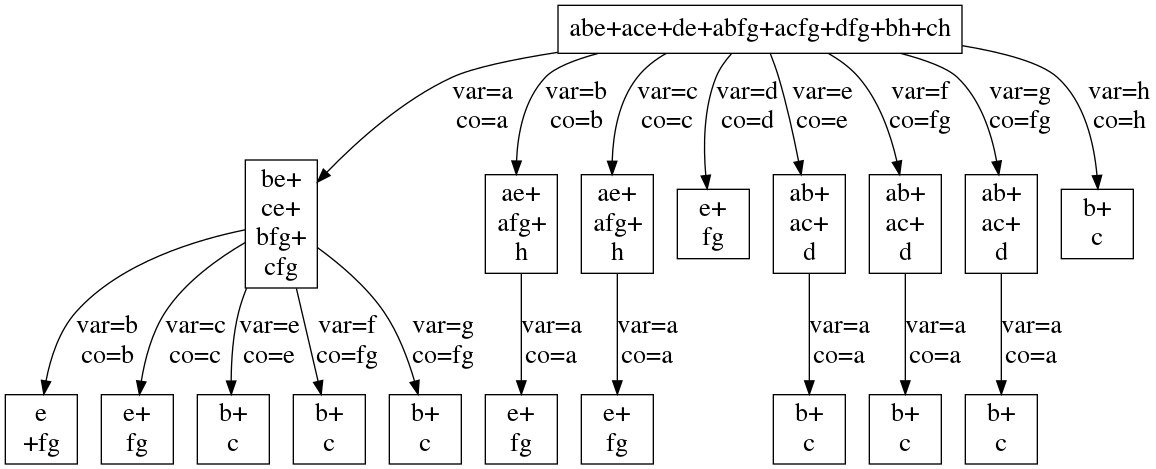
\includegraphics[width = 6.50in, height = 2.80in]{kernel.png}
\end{center}

All the kernel --- co-kernel pairs are shown in the table:
\begin{center}
    \tabcolsep=8pt
    \begin{tabular}{|c|c|c|}
        \hline
        kernel & co-kernel & level of kernel \\
        \hline
        $abe+ace+de+abfg+acfg+dfg+bh+ch$ & 1                    & 2 \\
        $be+ce+bfg+cfg$                  & $a$                  & 1 \\ 
        $ae+afg+h$                       & $b$ or $c$           & 1 \\
        $ab+ac+d$                        & $e$ or $fg$          & 1 \\
        $b+c$                            & $h$ or $ae$ or $afg$ & 0 \\
        $e+fg$                           & $d$ or $ab$ or $ac$  & 0 \\
        \hline
    \end{tabular}
\end{center}

\section{(18\%) Single Cube Divisor Extraction}
Consider the following Boolean logic network with variables $a$, $b$, $c$, $d$, $e$, $f$:
\[R=abf+abcd+abce+cdf\]
\[S=acd+cdef+abce\]
\[T=cdef+af\]

Build the cube-literal matrix associated with this set of functions.
List all the single cube divisors that can be extracted based on a non-trival prime rectangle that covers the column $c$.
(Here, a prime rectangle is non-trival if it covers at least two rows and at least two column.)
Which of them are the best in terms of the number of literals saved?
You should apply the simple formula talked in lecture to compute the number of literals saved.\\

Answer:

The cube-literal matrix is shown in the table:
\begin{center}
    \tabcolsep=8pt
    \begin{tabular}{|c|cccccc|}
        \hline
        & $a$ & $b$ & $c$ & $d$ & $e$ & $f$ \\
        \hline
        $abf$  & 1 & 1 & - & - & - & 1 \\
        $abcd$ & 1 & 1 & 1 & 1 & - & - \\
        $abce$ & 1 & 1 & 1 & - & 1 & - \\
        $cdf$  & - & - & 1 & 1 & - & 1 \\
        $acd$  & 1 & - & 1 & 1 & - & - \\
        $cdef$ & - & - & 1 & 1 & 1 & 1 \\
        $af$   & 1 & - & - & - & - & 1 \\
        \hline
    \end{tabular}
\end{center}
All the single cube divisors are listed below:
\begin{center}
    \tabcolsep=8pt
    \begin{tabular}{|c|ccc|}
        \hline
        divisors & $C$   & $\sum Weight(r)$ & \# saved literals \\
        \hline
        $ac$     & $2$   & $1+2+1=4  $  & $(2-1)\times 4-2=2$\\
        $bc$     & $2$   & $1+2=3    $  & $(2-1)\times 3-2=1$\\
        $cd$     & $2$   & $1+1+1+2=5$  & $(2-1)\times 5-2=3$\\
        $ce$     & $2$   & $2+2=4    $  & $(2-1)\times 4-2=2$\\
        $cf$     & $2$   & $1+2=3    $  & $(2-1)\times 3-2=1$\\
        $abc$    & $3$   & $1+2=3    $  & $(3-1)\times 3-3=3$\\
        $acd$    & $3$   & $1+1=2    $  & $(3-1)\times 2-3=1$\\
        $cdf$    & $3$   & $1+2=3    $  & $(3-1)\times 3-3=3$\\
        \hline
    \end{tabular}
\end{center}

\section{(18\%) Multiple Cube Divisor Extraction}
Suppose that we have the following two Boolean functions,
defined over 9 variables $p$, $q$, $r$, $s$, $t$, $u$, $v$, $w$, $x$:
\[G=qt+rst+pqr+quvw+rsuvw\]
\[H=pu+qtx+qu+rsu\]
Apply the method we talked in the lecture to build a co-kernel-cube matrix.
List all multiple cube divisors that can be extracted based on a non-trivial prime rectangle.
(Here, a prime rectangle is non-trivial if it covers at least two rows and at least two columns.)
For each multiple cube divisor you have extracted,
draw the the Boolean network.
What is the number of literals saved with each extracted multiple cube divisor?
You should apply the simple formula talked in lecture to compute the number of literals saved.

To assist you in the construction,
here are all the kernels and co-kernels for the two functions:

Function $G=qt+rst+pqr+quvw+rsuvw$
\begin{center}
    \tabcolsep=8pt
    \begin{tabular}{|c|c|}
        \hline
        Kernel & Co-kernel \\
        \hline
        $t+pr+uvw$   & $q$   \\
        $t+uvw$      & $rs$  \\
        $st+pq+suvw$ & $r$   \\
        $q+rs$       & $t$   \\
        $q+rs$       & $uvw$ \\
        \hline
    \end{tabular}
\end{center}

Function $H=pu+qtx+qu+rsu$
\begin{center}
    \tabcolsep=8pt
    \begin{tabular}{|c|c|}
        \hline
        Kernel & Co-kernel \\
        \hline
        $u+tx$       & $q$   \\
        $p+q+rs$     & $u$   \\
        \hline
    \end{tabular}
\end{center}

Answer:

The co-kernel-cube matrix is:
\begin{center}
    \tabcolsep=8pt
    \begin{tabular}{|c|ccccccccccc|}
        \hline
                  & $t$ & $p$ & $q$ & $u$ & $pr$ & $st$ & $pq$ & $rs$ & $tx$ & $uvw$ & $suvw$ \\
        \hline
        $G$ $q$   & 1   & -  &  -   & -   & 1    & -    & -    & -    & -    & 1     & -      \\
        $G$ $rs$  & 1   & -  &  -   & -   & -    & -    & -    & -    & -    & 1     & -      \\
        $G$ $r$   & -   & -  &  -   & -   & -    & 1    & 1    & -    & -    & -     & 1      \\
        $G$ $t$   & -   & -  &  1   & -   & -    & -    & -    & 1    & -    & -     & -      \\
        $G$ $uvw$ & -   & -  &  1   & -   & -    & -    & -    & 1    & -    & -     & -      \\
        $H$ $q$   & -   & -  &  -   & 1   & -    & -    & -    & -    & 1    & -     & -      \\
        $H$ $u$   & -   & 1  &  1   & -   & -    & -    & -    & 1    & -    & -     & -      \\
        \hline
    \end{tabular}
\end{center}

All multiple cube divisors are $t+uvw$ and $q+rs$.

For $t+uvw$:
\[G=(t+uvw)(q+rs)+pqr\]
\[H=pu+qtx+qu+rsu\]
\begin{center}
    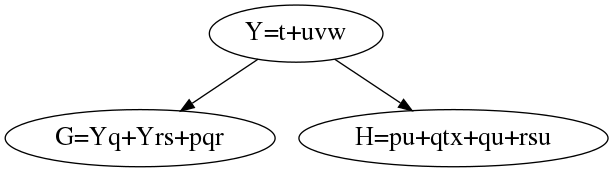
\includegraphics[width = 3.50in, height = 1.00in]{t_add_uvw.png}
\end{center}
Column weight,
\[Weight(t)=1\]
\[Weight(uvw)=3\]
Row weight,
\[Weight(G q)=1+1=2\]
\[Weight(G rs)=1+2=3\]
$\sum{Value(r,c)}$,
\[2+4+3+5=14\]
\# literals saved:
\[14-(3+2)-(1+3)=5\]
For $q+rs$:
\[G=(q+rs)(t+uvw)+pqr\]
\[H=(q+rs)(u)+pu+qtx\]
\begin{center}
    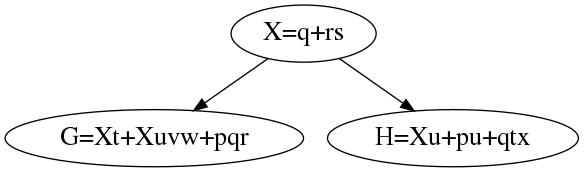
\includegraphics[width = 3.50in, height = 1.00in]{q_add_rs.png}
\end{center}
Column weight,
\[Weight(q)=1\]
\[Weight(rs)=2\]
Row weight,
\[Weight(G t)=1+1=2\]
\[Weight(G uvw)=1+3=4\]
\[Weight(H u)=1+1=2\]
$\sum{Value(r,c)}$,
\[2+3+4+5+2+3=19\]
\# literals saved:
\[19-(1+2)-(2+4+2)=8\]

\section{(10\%) Controllability Don't Cares (CDCs) in Multi-Level Logic}
Consider the following small Boolean logic network:
\begin{center}
    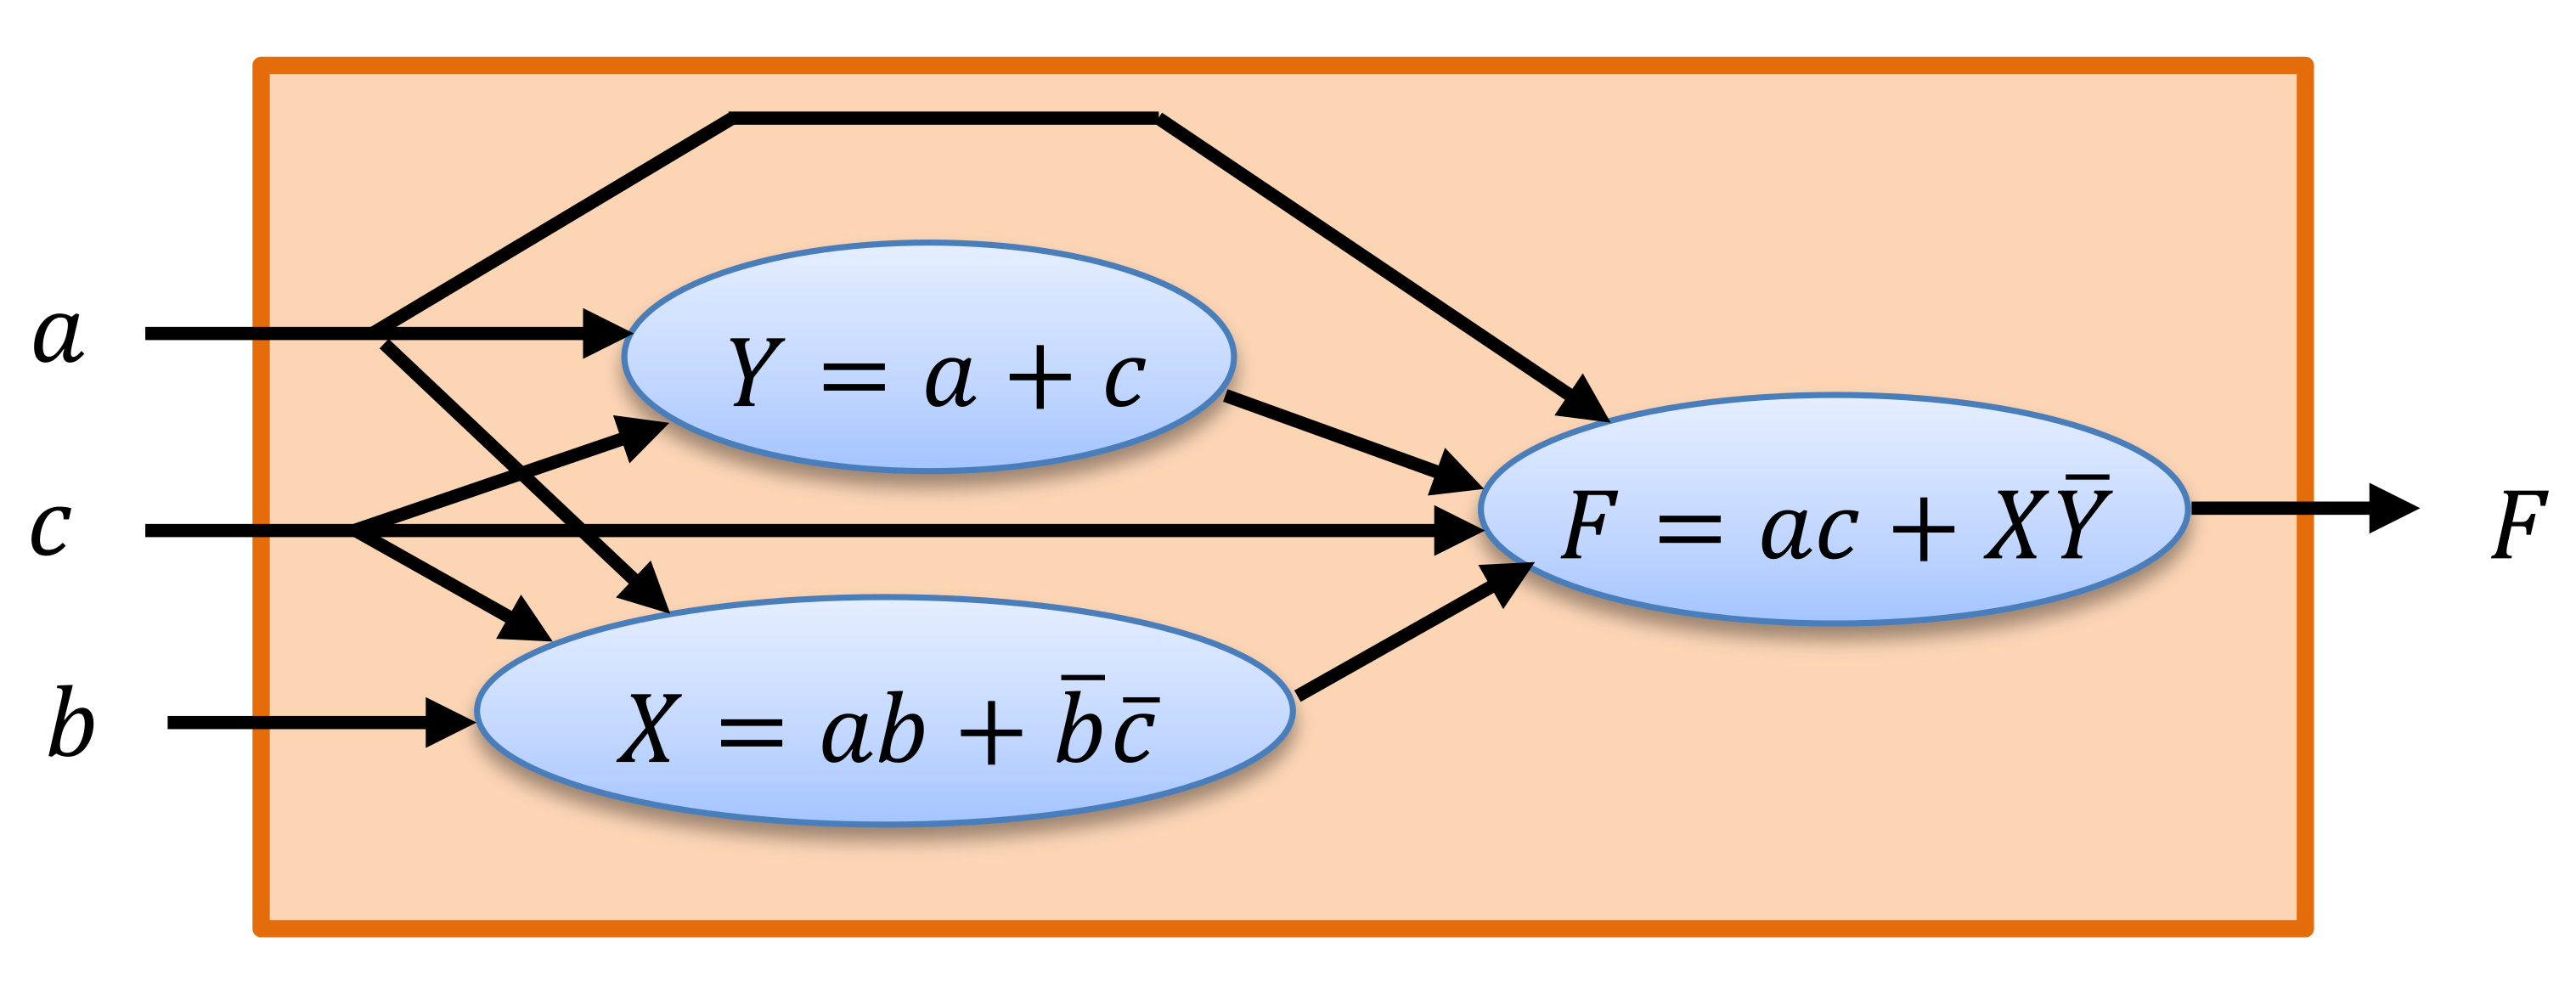
\includegraphics[width = 5.50in, height = 2.00in]{cdc.png}
\end{center}

Use the methods from the lecture to obtain $CDC_F$ for node F.

Answer:

The inputs of $F$ are $X$, $Y$, $a$ and $c$.
Their SDCs are:
\[SDC_X=X\oplus{(ab+\bar{b}\bar{c})}\]
\[SDC_Y=Y\oplus{(a+c)}\]
\[SDC_a=0\]
\[SDC_c=0\]
$b$ is not used in $F$.
\[
\begin{split}
    & CDC_F= \\
    & (\forall{b})[SDC_X+SDC_Y]= \\
    & (\forall{b})[X\oplus{(ab+\bar{b}\bar{c})} + Y\oplus{(a+c)}]= \\
    & [X\oplus{(ab+\bar{b}\bar{c})} + Y\oplus{(a+c)}]_{b=1}\cdot [X\oplus{(ab+\bar{b}\bar{c})} + Y\oplus{(a+c)}]_{b=0} = \\
    & [(X\oplus{a}) + (Y\oplus{(a+c)})]\cdot [(X\oplus{\bar{c}}) + (Y\oplus{(a+c)})] = \\
    & (Y\oplus{(a+c)}) + (X\oplus{a})(X\oplus{\bar{c}}) = \\
    & Y\bar{a}\bar{c} + \bar{Y}a + \bar{Y}c + X\bar{a}c + \bar{X}a\bar{c}
\end{split}
\]

\section{(8\%) Observability Don't Cares (ODCs) in Multi-Level Logic}
Condider the following small Boolean logic network:
\begin{center}
    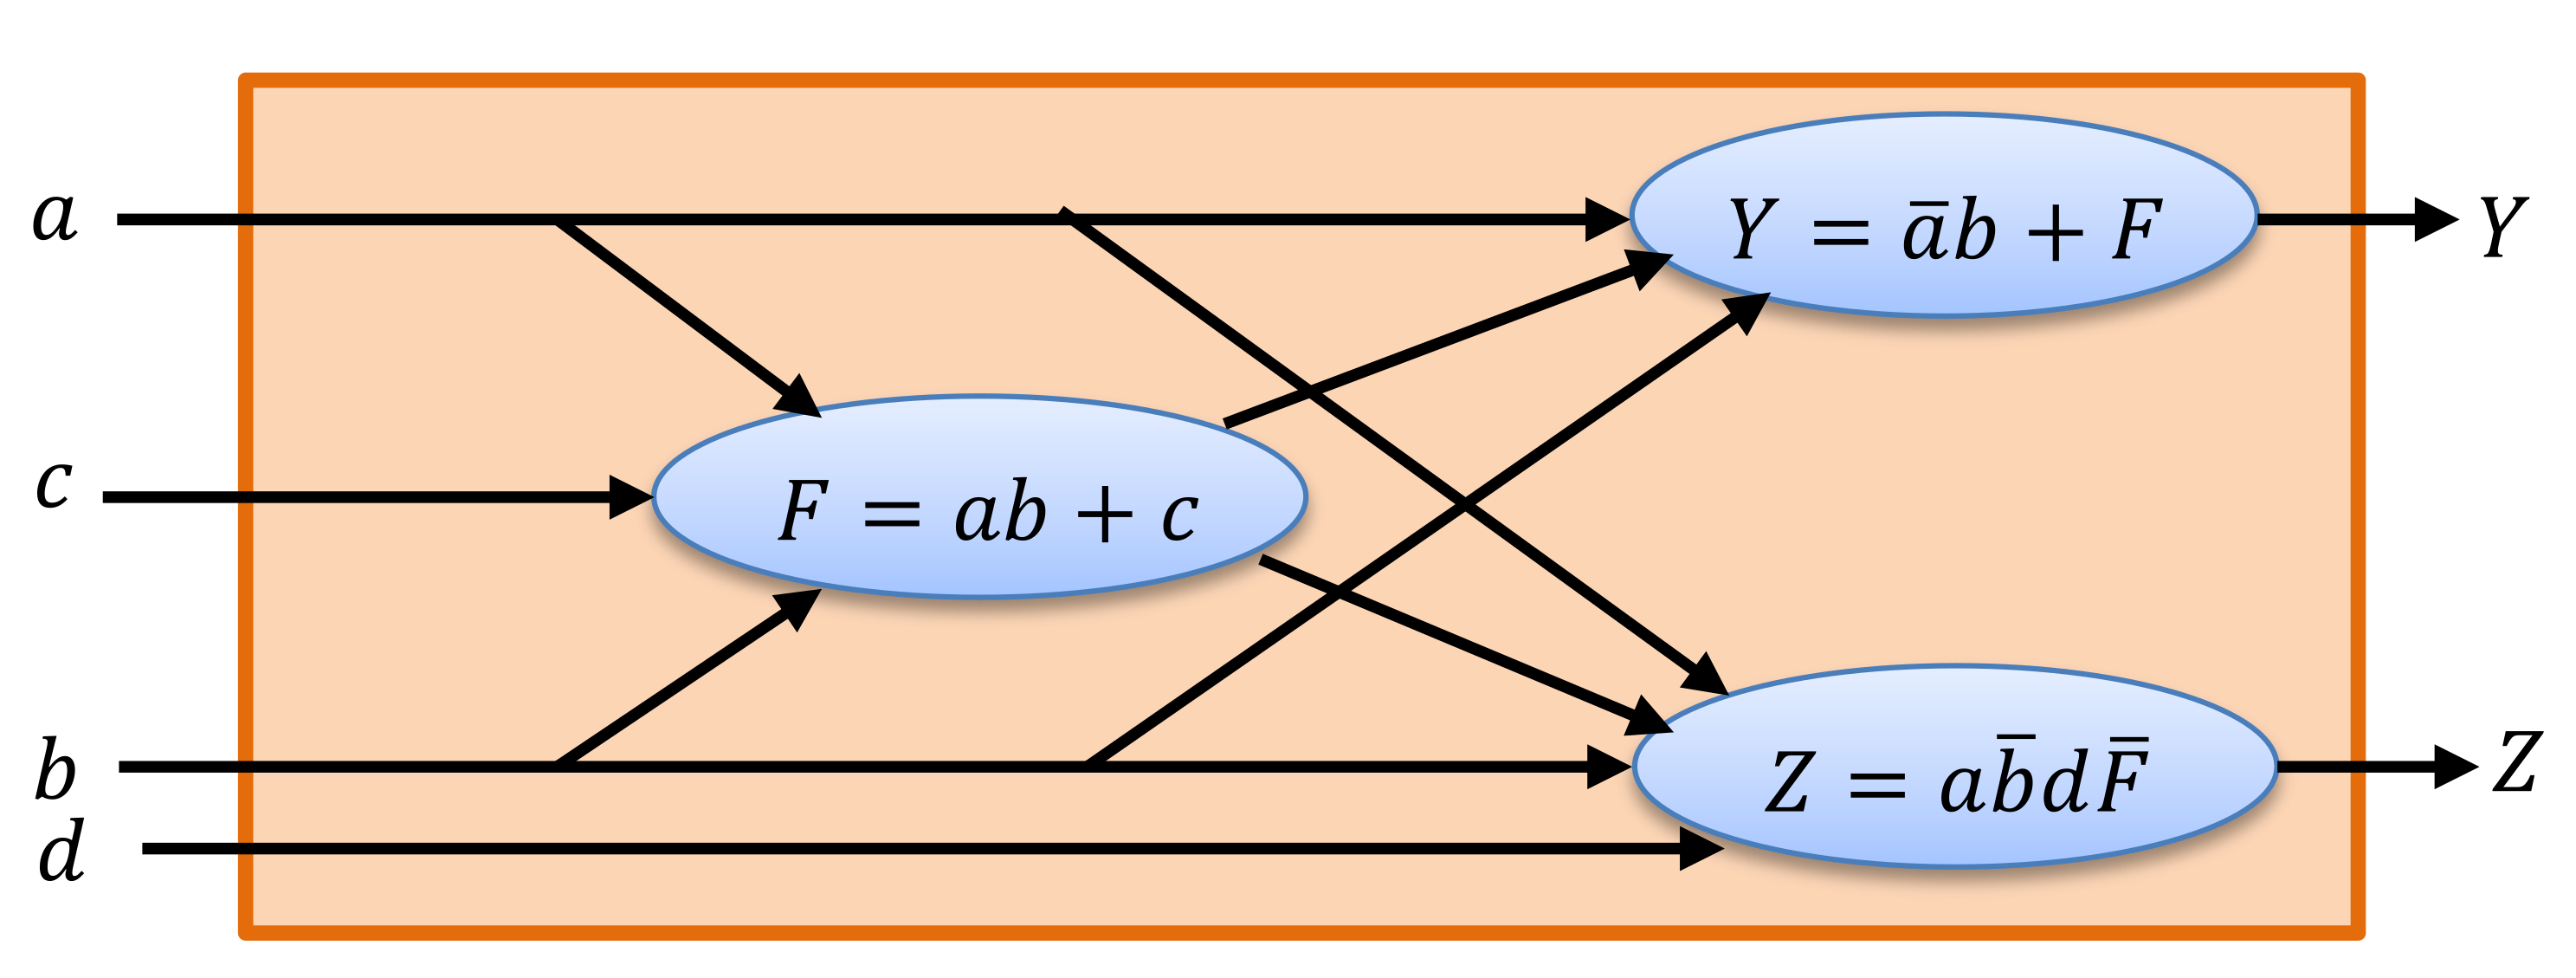
\includegraphics[width = 5.50in, height = 2.00in]{odc.png}
\end{center}

Use the methods from the lecture to obtain $ODC_F$ for node F.

Answer:

The outputs of $F$ are $Y$ and $Z$.
The negation of Boolean difference are:
\[\overline{\partial{Y}/\partial F} = (\bar{a}b) \overline\oplus 1 = \bar{a}b\]
\[\overline{\partial{Z}/\partial F} = (a\bar{b}d) \overline\oplus 0 = \bar{a}+b+\bar{d}\]
\[\overline{\partial{Y}/\partial F}\cdot \overline{\partial{Z}/\partial F} = \bar{a}b + \bar{a}b\bar{d}\]
$d$ is not used in $F$.
\[
    \begin{split}
        & ODC_F = \\
        & (\forall{d})[\overline{\partial{Y}/\partial F}\cdot \overline{\partial{Z}/\partial F}] = \\
        & (\forall{d})[\bar{a}b + \bar{a}b\bar{d}] = \\
        & [\bar{a}b] \cdot [\bar{a}b] = \\
        & \bar{a}b 
    \end{split}
\]

\end{document}
